\chapter{Advanced topics on \RV}

Objectives of this chapter are
\begin{enumerate}
    \item deriving the distribution of a function of a \rv(s)
    \item sum of independent \rv and also where the number of \rv is itself random
    \item quantifying the degree of dependence between \rv
\end{enumerate}

\section{Derived Distributions}
Given a continuous \rv $X$ we want to calculate PDF of a \rv $Y=g(X)$ (also called as \textit{derived distribution}). The two step cookbook procedure is as follows:
\begin{enumerate}
    \item Calculate the CDF $F_Y(y)$ using:
    \[F_Y(y)=P(g(X)\le y)=\int_{\{x|g(X)\le y\}}f_X(x) dx\]
    \item Differentiate to obtain the PDF of Y:
    \[f_Y(y)=\frac{d \, F_Y}{dy}(y)\]
\end{enumerate}
More concisely it can be written as:
\begin{center}
    PDF of X $\to$ CDF of X $\to$ CDF of Y $\to$ PDF of Y
\end{center}

\subsection{PDF of a Linear Function of a \RV}
Let $X$ be a continuous \rv with PDF $f_X$ and let $Y=aX+b$ where $a \neq 0$ and $b$ are scalars. Then
\[\boxed{f_Y(y)=\frac{1}{|a|}f_X\left( \frac{y-b}{a}\right)}\]

\begin{remark}
    This equation can be used in proving that the linear function of a Normal \RV is also Normal.
\end{remark}

\subsection{Monotonic Functions}
Suppose that $g$ is strictly monotonic with inverse $h$. Assume that $h$ is differentiable, then the PDF of $Y =g(X)$ in the region where $f_Y(y)>0$ is given by
\[\boxed{f_Y(y)=f_X(h(y)) \left| \frac{dh}{dy}(y) \right|}\]

\subsubsection{Proof}
Suppose that $g$ is monotonically increasing
\[F_Y(y)=P(g(X)\le y)=P(X\le h(y))=F_X(h(y))\]
Differentiating to obtain PDF of Y using chain rule we get
\[f_Y(y)=\frac{dF_Y}{dy}(y)=f_X(h(y))\frac{dh}{dy}(y)\]
Because $g$ is monotonically increasing so will be $h$ so its derivative is non-negative. So the rule follows.

For monotonically decreasing case, we get
\[F_Y(y)=P(g(X)\le y)=P(X \ge h(y))=1-F_X(h(y))\]
and use the chain rule to obtain the above relation.
\qed

\subsubsection{Intuition}

\begin{figure}[h]
    \center
    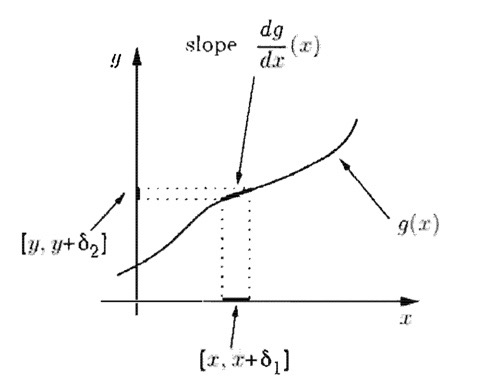
\includegraphics[width=.5\textwidth]{images/P_4_derived_distribution.jpeg}
 \end{figure}

 Consider a small interval $[x,x+\delta_1], \delta_1 \approx 0$ and a monotonically increasing function $g$. The image of this interval is the interval $[y, y+\delta_2]$. We have following based on the slope
 \[\frac{\delta_2}{\delta_1} \approx \frac{dg}{dx}(x)\]
 or in terms of inverse function
 \[\frac{\delta_1}{\delta_2}\approx \frac{dh}{dy}(y)\]

 Note that the event $\{x \le X \le x+\delta_1\}$ is same as the event $\{y\le Y \le y+\delta_2\}$. Thus,
 \begin{align*}
     f_Y(y)\delta_2 & \approx P(y\le Y \le y+\delta_2) \\
          &= P(x \le X \le x+\delta_1) \\
          &= f_X(x)\delta_1
 \end{align*}

This leads to following two relations
 \[f_X(x)=f_Y(y) \cdot \frac{\delta_2}{\delta_1}=f_Y(y)\frac{dg}{dx}(x), \qquad f_Y(y)=f_X(h(y))\cdot \frac{\delta_1}{\delta_2}=\frac{dh}{dy}(y)\]

 \subsection{Function of Two \RV}
 The same cookbook procedure of first finding the CDF and then differentiating it to get PDF also applies when there are multiple \rv

\subsubsection{Example: Romeo \& Juliet}
Romeo and Juliet have a date at a given time and they are late by amount of time (independently of each other) that is exponentially distributed with parameter $\lambda$. What is the PDF of their differences in time of arrival?


Let us denote by $X$ and $Y$ the amount of time by which Romeo and Juliet are late respectively. We want to calculate PDF of $Z=X-Y$. We'll calculate CDF $F_Z(z)$ by considering the cases $z\ge 0$ and $z<0$.
For $z\ge 0$, we have,
\begin{align*}
    F_Z(z) &= P(X-Y \le z) \\
           &= 1 - P(X-Y>z) \\
           &= 1 - \int_{z}^{\infty} \lambda e^{-\lambda x} \left(\int_{0}^{x-z} \lambda e^{-\lambda y} dy \right) dx \\
           &= 1 - \frac{1}{2} e^{-\lambda z}
\end{align*}
For the case $z<0$, we can have a similar calculation but we'll argue in terms of symmetry of the situation. The variables $Z=X-Y$ and $-Z=Y-X$ have the same distribution. We have
\[F_Z(z) = P(Z \le z) = P(-Z\ge -z) = P(Z\ge -z)= 1 - F_Z(-z)=\frac{1}{2} e^{\lambda z}\]

Thus after differentiating the CDF we get the PDF as 
\[f_Z(z) = \frac{\lambda}{2}e^{-\lambda |z|}\]
This is also called as two-sided exponential PDF or Laplace PDF.
\qed

\subsection{Sums of many Independent \RV (Convolution)}
Let $Z=X+Y$ where $X,Y$ be two independent discrete \rv with PMFs $p_X$ and $p_Y$ respectively. Then for any integer $z$,
\begin{align*}
    p_Z(z) &= P(X+Y=z) \\
           &= \sum_{\{(x,y)|x+y=z \}} P(X=x, Y=y) \\
           &= \sum_xP(X=x, Y=z-x) \\
           &= \sum_x p_X(x)p_Y(z-x)
\end{align*}

The resulting PMF $p_Z$ is called as the convolution of PMFs of $X$ and $Y$.

Suppose now that $X$ and $Y$ are independent continuous \rv and we want to find the PDF of $Z=X+Y$.

Note that
\[P(Z\le z|X=x) = P(X+Y\le z|X=x) = P(Y\le z-x)\]

The last equality follows because of independence of $X$ and $Y$.We differentiate both sides w.r.t. $z$ and find that $f_{Z|x}(z|x)=f_Y(z-x)$. Using multiplication rule we get

\[f_{X,Z}(x,z)=f_X(x)f_{Z|X}(z|x)=f_X(x)f_Y(z-x)\]

Finally we obtain
\[f_Z(z)=\int_{-\infty}^{\infty}f_{X,Z}(x,z) dx = \int_{-\infty}^{\infty}f_X(x)f_Y(z-x) dx\]

\subsubsection{Intuition}
\begin{figure}[h]
    \center
    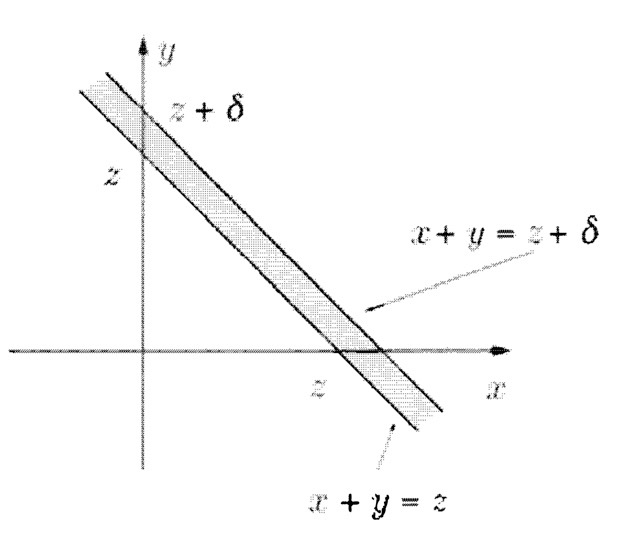
\includegraphics[width=.4\textwidth]{images/P_4_convolution.jpeg}
 \end{figure}

 Consider the strip as shown in the figure with small $\delta$.The probability of the strip is $P(z \le X+Y \le z+\delta) \approx f_Z(z) \delta$
 \begin{align*}
    f_Z(z) \delta &= P(z \le X+Y \le z+\delta) \\
    &= \int_{-\infty}^{\infty}\int_{z-x}^{z-x+\delta} f_X(x)f_Y(y) \, dy \, dx \\
    & \approx \int_{-\infty}^{\infty}f_X(x)f_Y(z-x) \delta \, dx
 \end{align*}
 Canceling $\delta$ on both sides gives the desired result. \qed
 \newline
 \begin{remark}
    Sum or of two normal \rv is normal and scalar multiple of a normal \rv is also normal, therefore for normal \rv $X, Y$ the \rv $aX+bY$ is also normal. 
 \end{remark}

 \subsubsection{Example: Romeo \& Juliet (Difference of \RV)}
 Here's a different solution using convolution.

 Note that the difference of \rv $X-Y$ can be viewed as $X+(-Y)$. We observe that $f_{-Y}(y)=f_Y(-y)$.
 \begin{align*}
     f_{X-Y}(z) &= \int_{-\infty}^{\infty}f_X(x)f_{-Y}(z-x) \, dx \\
      &= \int_{-\infty}^{\infty}f_X(x)f_Y(x-z) \, dx \\
      &= \int_{z}^{\infty} \lambda e^{-\lambda x} \lambda e^{-\lambda(x-z)} \, dx\\
      &= \lambda^2 e^{\lambda z} \int_{z}^{\infty} e^{-2 \lambda x} \, dx \\
      &= \frac{\lambda}{2} e^{-\lambda z}
 \end{align*}
 The answer for the case $z<0$ is obtained using symmetry, since $X, Y$ are identically distributed,
 \[f_{X-Y}(z)=f_{Y-X}(z)=f_{-(X-Y)}(z)=f_{X-Y}(-z)\] \qed

 \subsection{Graphical Calculation of Convolution}

 Let $t$ be a dummy variable and suppose that we have two PDFs $f_X(t)$ and $f_Y(t)$. The graphical evaluation consists of the following steps:
 \begin{enumerate}
     \item We plot $f_Y(z-t)$ as a function of $t$. The plot has the same shape as that of $f_Y(t)$ but first flipped and then shifted to left/right depending whether $z<0$ or $z>0$.
     \item We place the plots of $f_X(t)$ and $f_Y(z-t)$ on top of each other and form their product.
     \item We calculate $f_Z(z)$ by calculating the integral of the product of the plots.
 \end{enumerate}

 By varying the amount of shifting as controlled by $z$ we can calculate for any $z$.

 \section{Covariance and Correlation}
 The covariance of two \rv $X, Y$ is denoted by cov$(X,Y)$ and is defined as
 \[\boxed{\text{cov}(X,Y)=\E\big[(X-\E[X])(Y-\E[Y])\big]}\]
 A zero covariance means that the \rv are uncorrelated. A positive covariance means that the values of $X-\E[X]$ and $Y-\E[Y]$ obtained in a single experiment "tend" to have same sign.

 \begin{remark}
    If $X, Y$ are independent then the covariance is zero but the converse may not be true.
 \end{remark}

 An alternative formula is 
 \[\boxed{\text{cov}(X,Y)=\E[XY]-\E[X]\E[Y]}\]

 Simple properties of covariances are
 \begin{align*}
     \text{cov}(X,X) &= \text{var}(X) \\
     \text{cov}(X, aY+b) &= a \cdot \text{cov}(X, Y) \\
     \text{cov}(X, Y+Z) &=\text{cov}(X,Y)+\text{cov}(X,Z)
 \end{align*}

 The \textbf{correlation coefficient} $\rho(X,Y) \in [-1, 1]$ is defined as 
 \[\boxed {\rho(X,Y) =\frac{\text{cov}(X,Y)}{\sqrt{\text{var}(X) \text{var}(Y)}} }\]

 \subsection{Variance of Sum of \RV}
 The covariance can be used to calculate the variance of sum of several \rv (not necessarily independent). In particular if $X_1, \ldots, X_n$ are \rv with finite variances, then
 \[\text{var}(X_1+X_2)=\text{var}(X_1)+\text{var}(X_2)+2\text{cov}(X_1, X_2)\]
 or more generally
 \[\text{var}\left(\sum_{i=1}^{n}X_i\right)=\sum_{i=1}^n\text{var}(X_i) + \sum_{i \neq j}\text{cov}(X_i, X_j)\]

 \section{Iterated Expectations}
 We revisit the conditional expectation of a \rv $X$ given another \rv $Y$ and we treat it as a \rv whose value is determined by $Y$.

 We define $\E[X|Y]$ to be a \rv that takes the value $\E[X|Y=y]$ when $Y$ takes a value $y$. Since $\E[X|Y=y]$ is a function of $y$, $\E[X|Y]$ is a \textit{function} of $Y$.

 Since $\E[X|Y]$ is a \rv it has expectation of its own,
 \[ \E[\E[X|Y]] = \E[X] = \begin{cases}
    \displaystyle\sum_y p_Y(y) \E[X|Y=y], & Y \text{ discrete} \\
    \displaystyle\int_{-\infty}^\infty f_Y(y)\E[X|Y=y] \, dy, & Y \text{ continuous}
 \end{cases} \]

 The equality is also called as 
 \[\boxed{ \textbf{Law of Iterated Expectations:} \quad \E[\E[X|Y]]=\E[X] }\]

 This law is the abstract notation of the total expectation theorem which loosely says that the average in whole is the weighted average of the parts where weights are the probabilities.
 
 For a function $g$, the following property holds (because $g(Y)$ will be a constant)
 \[\E[Xg(Y)|Y]=g(Y)\E[X|Y]\]

 \subsection{Conditional Expectation as an Estimator}
 If $Y$ provides information about $X$ then $\hat X = \E[X|Y]$ is an estimator for $X$ given $Y$. The estimation error is $\tilde X = \hat X - X$ that satisfies
 \[\E[\tilde X | Y]=\E[\hat X - X |Y]=\E[\hat X|Y]-\E[X|Y]=\hat X - \hat X = 0\]

 Thus the \rv $\E[\tilde X |Y]$ is identically zero. By using law of iterated expectations $\E[\tilde X]=\E[\E[\tilde X|Y]]=0$. This reassures that the estimation error doesn't have any systematic upward or downward bias.

 We now show that $\tilde X$ is uncorrelated with $\hat X$. Using law of iterated expectations
 \[\E[\tilde X \hat X]=\E[\E[\tilde X \hat X|Y]]=\E[\hat X \E[\tilde X|Y]]=0\]
 where the last two equality follows because $\hat X$ is completely determined by $Y$. It follows that 
 \[\text{cov}(\tilde X,\hat X)=\E[\tilde X \hat X]-\E[\tilde X]\E[\hat X] = 0 - \E[\hat X] \cdot 0=0\]
 Thus $\hat X$ and $\tilde X$ are uncorrelated.

 \subsection{Conditional Variance}
 We introduce the \rv 
 \[\text{var}(X|Y)=\E \big [(X-\E[X|Y])^2 \, | \,Y \big ]=\E[\tilde X ^2 | Y]\]
 using the fact that $\E[\tilde X]=0$ and the law of iterated expectations, the variance of the estimation error is
 \[\var(\tilde X)=\E[\tilde X ^2]=\E[\E[\tilde X ^2|Y]]=\E[\var(X|Y)]\]

 Therefore $\var(X)=\var(\tilde X) + \var(\hat X)$ which gives us
 \[\boxed{ \textbf{Law of Total Variance:} \quad \var(X)=\E[\var(X|Y)]+\var(\E[X|Y])}\]

 \subsubsection{Intuitive Example}
 Suppose that we want to find the total variance of quiz scores of a class. Suppose that $X$ is the quiz score of the student and $Y\in \{1,\ldots,k\}$ denotes the section of the student.
 
 Let $n_s$ be the number of students in section $s$ and $n$ be the total number of students. We interpret the total variance formula as:
 \begin{enumerate}
     \item $\E[\var(X|Y)]$ is the variability within the sections and is the weighted average of section variances where the weight is proportional to its size.

     $\var(X|Y=s)$ is the variance of quiz scores \textit{within} section $s$. Thus
     \[\E[\var(X|Y)]=\sum_{s=1}^{k}P(Y=s)\var(X|Y=s)=\sum_{s=1}^{k}\frac{n_s}{n}\var(X|Y=s)\]
     \item $\var(\E[X|Y])$ is the variability of the average scores ($\E[X|Y]$) \textit{between} the sections.
 \end{enumerate}

 Combining the values we get $\var(X)=\var(\E[X|Y])+\E[\var(X|Y)]$

 \section{Transform}

 \section{Sum of random number of independent random variables}

 We consider the sum
 \[Y=X_1+\cdots+X_N\]
 where $N$ is a \rv that takes non negative values and $X_i$'s are identically distributed random variables. We assume $N,X_1,\ldots$ are independent so that any finite subset of \rv are also independent. Let $E[X]$ and $\var(X)$ denote the common mean and variance, respectively, of the $X_i$.

 Fix a nonnegative integer $N=n$. Since the sum $X_1+\cdots+X_n$ is independent of $N$ and therefore is independent of $\{N=n\}$.
 \begin{align*}
    \E[Y|N=n] &= \E[X_1+\cdots+X_N|N=n] \\
    &= \E[X_1+\cdots+X_n|N=n] \\
    &= \E[X_1+\cdots+X_n] \\
    &= n\E[X]
 \end{align*}

 Since it is true for every nonnegative integer $n$, so $\E[Y|N]=N\E[X]$. Using law of iterated expectations we get
 \[\E[Y]=\E[\E[Y|N]]=\E[N\E[X]]=\E[N]\E[X]\]
 Similarly,
 \begin{align*}
    \var(Y|N=n) &= \var(X_1+\ldots+X_N|N=n) \\
    &= \var(X_1+\ldots+X_n|N=n) \\
    &= n \, \var(X)
 \end{align*}
 Since this is true for every $N$ we get $\var(Y|N)=N\var(X)$
 We now use law of total variance to obtain
 \begin{align*}
     \var(Y) &= \E[\var(Y|N)] + \var(\E[Y|N]) \\
     &= \E[N\var(X)] + \var(N\E[X]) \\
     &= \var(X)\E[N] + (\E[X])^2\var(N)
 \end{align*}

 \textbf{See the transform method on p. 241 and its examples}